\documentclass{article}
\usepackage{geometry}
\geometry{a4paper, margin=1in}
\usepackage{graphicx}
\usepackage{listings}
\usepackage{xcolor}
\usepackage[utf8]{inputenc}

\lstset{
    basicstyle=\ttfamily\small,
    breaklines=true,
    frame=single,
    language=C,
    keywordstyle=\color{blue},
    commentstyle=\color{green!50!black},
    stringstyle=\color{red}
}

\begin{document}

\title{Operating Systems Lab Assignment: Synchronization and Scheduling}
\author{Your Name}
\date{\today}
\maketitle

\section{Introduction}
This lab uses threads in C with mutexes and condition variables. I compiled everything with gcc -pthread on Linux.

\section{Exercise 1: Hello World}
\lstinputlisting{hello_world.c}
\textbf{Explanation}: The lock and condition variable werent initialized and main didnt wait for the child, so it could print before hello changed. I added the init calls and made main wait in a while loop until hello is 1.

\textbf{Analysis}: The mutex keeps both threads from using hello at the same time and the condition variable makes main wait. Now it always prints in the right order.

\textbf{Screenshot}:
\begin{figure}[h]
    \centering
    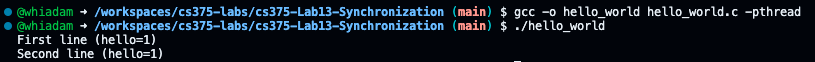
\includegraphics[width=\textwidth]{exercise1_screenshot.png}
    \caption{Compilation and execution of hello\_world.c}
\end{figure}

\section{Exercise 2: SpaceX Problems}
\lstinputlisting{spacex.c}
\textbf{Explanation}: The announcer could print before the countdown was done. Now it waits in a while loop until n is 0 and the counter signals every time it lowers n.

\textbf{Analysis}: The announcer keeps going back to sleep until n is 0, so the message always prints after 1.

\textbf{Screenshot}:
\begin{figure}[h]
    \centering
    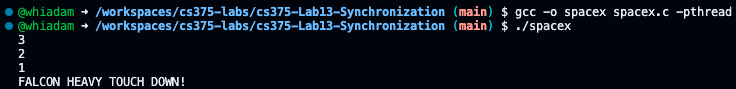
\includegraphics[width=\textwidth]{exercise2_screenshot.png}
    \caption{Compilation and execution of spacex.c}
\end{figure}

\section{Exercise 3: I Love You, Unconditionally!}
\lstinputlisting{love.c}
\textbf{Explanation}: Main could check subaru before the helper changed it and print I love Rem. Now main waits in a while loop until subaru is 1.

\textbf{Analysis}: It doesnt matter which thread runs first. The while loop rechecks the condition which is needed for Mesa semantics.

\textbf{Screenshot}:
\begin{figure}[h]
    \centering
    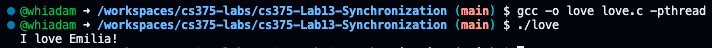
\includegraphics[width=\textwidth]{exercise3_screenshot.png}
    \caption{Compilation and execution of love.c}
\end{figure}

\section{Exercise 4: Locking Up the Floopies}
\lstinputlisting{floopy.c}
\textbf{Explanation}: Locking donor then recipient can deadlock if two transfers go opposite ways. Now it always locks the lower uuid first. I also added an args struct because the starter code passed the arguments wrong and could crash.

\textbf{Analysis}: Thread 1 locks account 1 and thread 2 locks account 2, then they both wait on each other forever. With the uuid order both threads go for account 1 first so that cant happen. Final balances were 900 and 600.

\textbf{Screenshot}:
\begin{figure}[h]
    \centering
    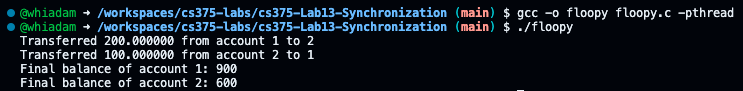
\includegraphics[width=\textwidth]{exercise4_screenshot.png}
    \caption{Compilation and execution of floopy.c}
\end{figure}

\section{Exercise 5: Baking with Condition Variables}
\lstinputlisting{baking.c}
\textbf{Explanation}: There are threads for batter, eggs, heating and eating that share one lock and three condition variables. I filled in the waits and signals and added some printfs.

\textbf{Analysis}: Nothing can be added while a cake is in the bowl and the heater waits for 1 batter and 2 eggs. It runs forever so I used head to show the first 20 lines.

\textbf{Screenshot}:
\begin{figure}[h]
    \centering
    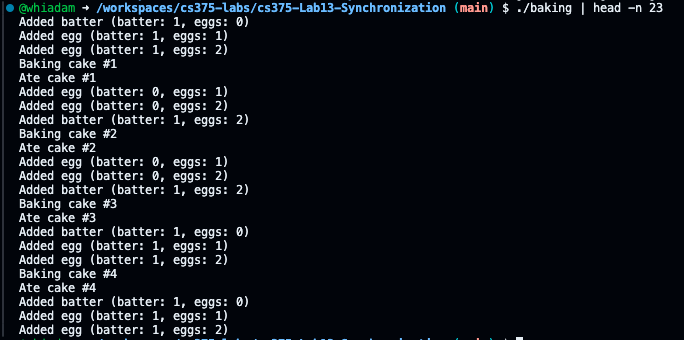
\includegraphics[width=\textwidth]{exercise5_screenshot.png}
    \caption{Compilation and execution of baking.c}
\end{figure}

\section{Exercise 6: Priority Donation in Transfer}
\lstinputlisting{priority_transfer.c}
\textbf{Explanation}: Priority inversion is when a high priority thread waits on a lock held by a low priority one. When a thread gets blocked it gives its priority to the holder, and the holder resets it to 0 when its done.

\textbf{Analysis}: The output shows the priority 2 thread donating and the low thread running at priority 2 so it finishes faster. The accounts still lock in uuid order so there is no deadlock.

\textbf{Screenshot}:
\begin{figure}[h]
    \centering
    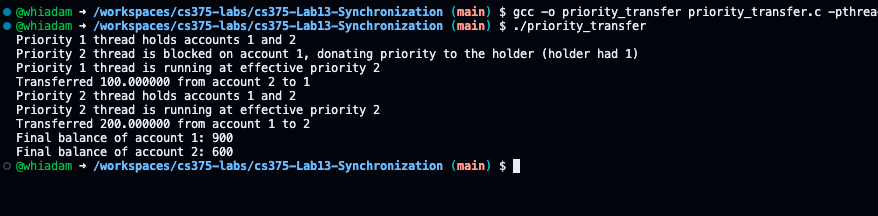
\includegraphics[width=\textwidth]{exercise6_screenshot.png}
    \caption{Compilation and execution of priority\_transfer.c}
\end{figure}

\section{Exercise 7: Barrier Synchronization}
\lstinputlisting{barrier.c}
\textbf{Explanation}: Each thread adds to count and waits until the last one gets there and broadcasts. I changed the if to a while loop with a generation number so threads cant leave early.

\textbf{Analysis}: All the Before barrier lines print before any After barrier lines. It needs broadcast because signal only wakes one thread.

\textbf{Screenshot}:
\begin{figure}[h]
    \centering
    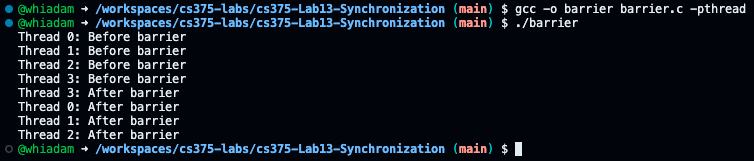
\includegraphics[width=\textwidth]{exercise7_screenshot.png}
    \caption{Compilation and execution of barrier.c}
\end{figure}

\section{Exercise 8: Readers-Writers with Priority}
\lstinputlisting{readers_writers.c}
\textbf{Explanation}: Readers wait if a writer is waiting, so writers get to go first. I changed signal to broadcast because the second writer could get stuck.

\textbf{Analysis}: Multiple readers can read at once but a writer goes alone. Readers could starve if writers keep coming.

\textbf{Screenshot}:
\begin{figure}[h]
    \centering
    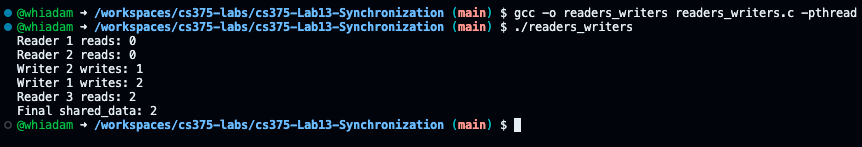
\includegraphics[width=\textwidth]{exercise8_screenshot.png}
    \caption{Compilation and execution of readers\_writers.c}
\end{figure}

\section{Exercise 9: Thread Pool}
\lstinputlisting{thread_pool.c}
\textbf{Explanation}: 4 worker threads take tasks from a queue protected by a mutex. I made pop wait on not\_empty instead of sleeping and added a shutdown flag so main can join the workers.

\textbf{Analysis}: Its faster than making a new thread for every task since the same 4 threads get reused. All 10 tasks ran once.

\textbf{Screenshot}:
\begin{figure}[h]
    \centering
    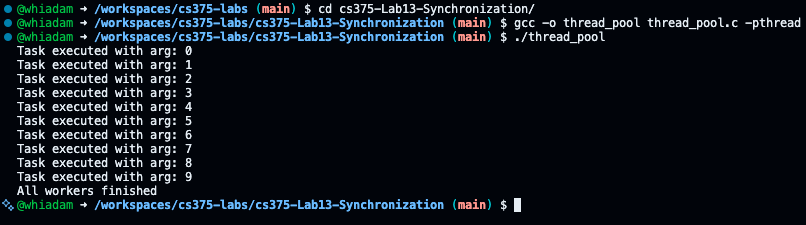
\includegraphics[width=\textwidth]{exercise9_screenshot.png}
    \caption{Compilation and execution of thread\_pool.c}
\end{figure}

\end{document}
